%! Author = jiang-ziyang
%! Date = 22-7-3

% Preamble
\documentclass{ctexart}

% Packages
\usepackage{graphicx}
\usepackage{epstopdf}
\usepackage{amsmath}
\usepackage{tikz}
\usepackage{ctex}
\usepackage{amssymb}
\usetikzlibrary{shapes,positioning}
\tikzstyle{inout}=[trapezium, trapezium left angle=60, trapezium right angle=120, draw] %%输入输出框
\tikzstyle{end}=[rectangle, rounded corners, draw]   %%教材上的起止框
\tikzstyle{endn}=[rounded rectangle, draw]   %%新版的起止框
\tikzstyle{exec}=[rectangle, draw]    %%执行框 execute
\tikzstyle{decide}=[kite, kite vertex angles=120, draw]   %%判断框


\title{一元二次方程在实数域上的求解}

\author{杨泽加 \\ 3190104662}

% Document
\begin{document}

    \maketitle
    \section{一元二次方程实数域上的求根公式及介绍}
    \begin{tabular}{p\columnwidth}
        一元二次方程的通式为
    \end{tabular}
    \begin{equation}\label{E1}
        f(x) = ax^2 + bx + c
    \end{equation}
    \begin{tabular}{p\columnwidth}
        对其求根有:
    \end{tabular}
    \begin{equation}\label{E2}
        \begin{aligned}
            ax^2 + bx + c &= 0\\
            x^2 + \frac{b}{a}x + \frac{c}{a} &= 0\\
            (x + \frac{b}{2a})^2 + (\frac{4ac - b^2}{4a^2}) &= 0\\
            (x + \frac{b}{2a})^2 &= (\frac{b^2 - 4ac}{4a^2}) \geqslant 0\\
            (if\ equation\ has\ a\ solution)
        \end{aligned}
    \end{equation}
    \begin{tabular}{p\columnwidth}
        则易得,当$ b^2 - 4ac \geqslant 0 $时方程有解且解为:
    \end{tabular}
    \begin{equation}\label{E3}
        x = \frac{-2ab \pm \sqrt {b^2 - 4ac}}{4a^2}
    \end{equation}
    \begin{tabular}{p\columnwidth}
        上式在$ b^2 - 4ac=0 $时退化为一个根 $-\frac{b}{2a}$。
    \end{tabular}
    \section{一元二次方程的求解算法流程图}\label{S1}
    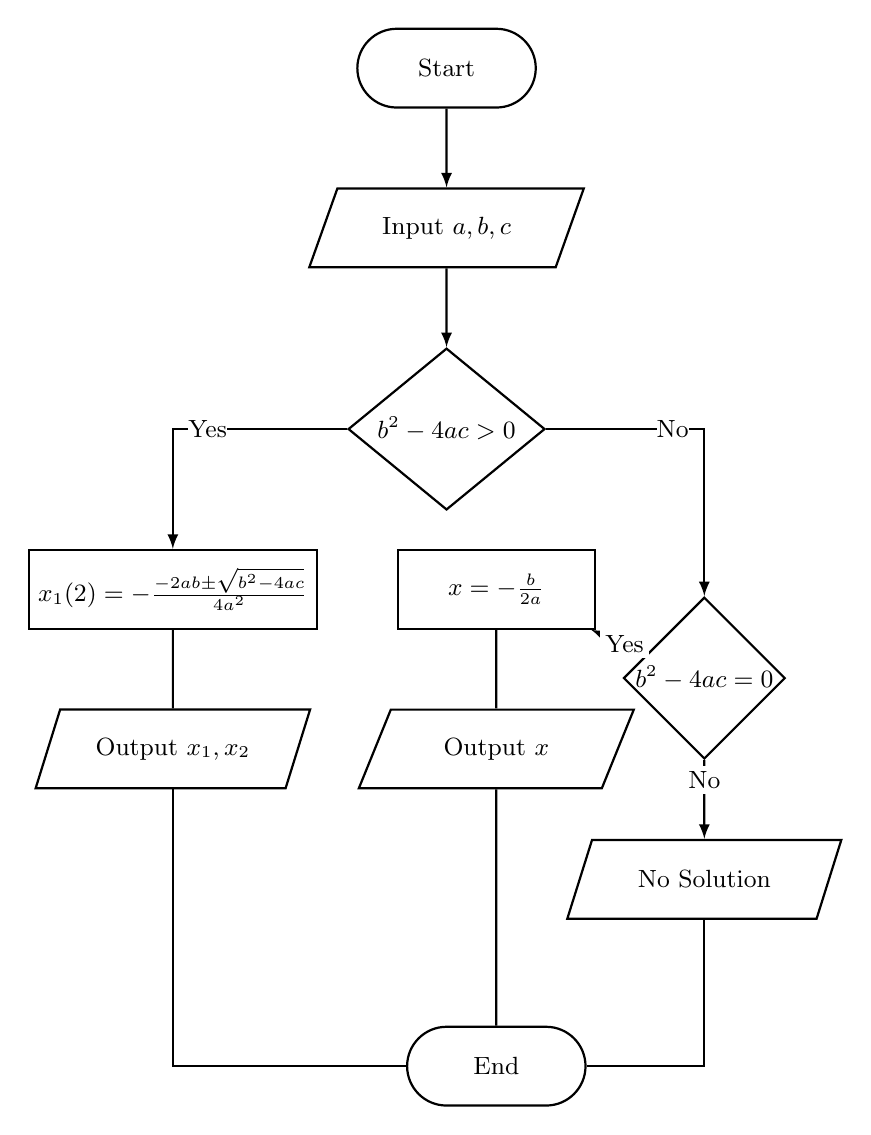
\begin{tikzpicture}[font=\small,thick]

        \node[draw,
            rounded rectangle,
            minimum width=2.5cm,
            minimum height=1cm] (block1) {Start};

        \node[draw,
            trapezium,
            trapezium left angle = 65,
            trapezium right angle = 115,
            trapezium stretches,
            below=of block1,
            minimum width=3.5cm,
            minimum height=1cm
        ] (block2) { Input $a,b,c$ };

        \node[draw,
            diamond,
            below=of block2,
            minimum width=2.5cm,
            inner sep=0
        ] (block3) { $b^2 - 4ac > 0$};

        \node[draw,
            diamond,
            below right =3cm of block3,
            inner sep=0] (block4) { $b^2 - 4ac = 0$};

        \node[draw,
            below left=of block3,
            minimum width=2.5cm,
            minimum height=1cm] (block5) { $x_1(2) = -\frac{-2ab\pm\sqrt {b^2 - 4ac}}{4a^2}$};

        \node[draw,
            left=of block4,
            right=of block5,
            minimum width=2.5cm,
            minimum height=1cm] (block6) { $x = -\frac{b}{2a}$};

        \node[draw,
            trapezium,
            trapezium left angle = 65,
            trapezium right angle = 115,
            trapezium stretches,
            below=of block5,
            minimum width=3.5cm,
            minimum height=1cm] (block7) { Output $x_1,x_2$};

        \node[draw,
            trapezium,
            trapezium left angle = 65,
            trapezium right angle = 115,
            trapezium stretches,
            below=of block6,
            minimum width=3.5cm,
            minimum height=1cm] (block8) { Output $x$};

        \node[draw,
            trapezium,
            trapezium left angle = 65,
            trapezium right angle = 115,
            trapezium stretches,
            below=of block4,
            minimum width=3.5cm,
            minimum height=1cm] (block9) { No Solution};

        \node[draw,
            rounded rectangle,
            below=3cm of block8,
            minimum width=2.5cm,
            minimum height=1cm,] (block10) {End};


% Arrows
        \draw[-latex] (block1) edge (block2)
        (block2) edge (block3);

        \draw[-latex] (block3) -| (block4)
        node[pos=0.4,fill=white,inner sep=0]{No};

        \draw[-latex] (block3) -| (block5)
        node[pos=0.4,fill=white,inner sep=0]{Yes};

        \draw[-latex] (block4) edge node[pos=0.4,fill=white,inner sep=2pt]{Yes}(block6)
        (block4) edge node[pos=0.25,fill=white,inner sep=2pt]{No} (block9);

        \draw (block5) edge (block7);
        \draw (block6) edge (block8);
        \draw (block7) |- (block10);
        \draw (block8) edge (block10);
        \draw (block9) |- (block10);

    \end{tikzpicture}

    \section{一元二次方程解的三种情况的示意图}\label{S2}

    \begin{figure}
        \centering
        \includegraphics{report_eps}
        \caption{生成文件的命令在文件 typescript 中}
        \label{l}
    \end{figure}

\end{document}